\begin{appendix}
\chapter{Algoritmo de Grover}\label{sec:Grover}

El algoritmo de Grover es el algoritmo cuántico de búsqueda óptimo en un conjunto desordenado \cite{grover1996fast}, \cite{nielsen2002quantum}. Lo llevamos a cabo con el operador de Grover $\hat{G}$ que es producto de dos operaciones en el espacio de n qubits $\hat{G}=(2\ket{\psi}\bra{\psi}-I)\hat{O}$: (1) el operador $\hat{O}:\ket{x}\xrightarrow{}(-1)^{f(x)}\ket{x}$, donde $f(x)$ es la función oráculo que tiene valor $f(x)=0$ cuando $x$ no es respuesta a la consulta (no es el elemento marcado), y $f(x)=1$ cuando $x$ sí es respuesta. $\hat{O}$ aplica un cambio de fase sobre los elementos marcados del conjunto. (2) el operador $2\ket{\psi}\bra{\psi}-I$ denomiado difusor de Grover.
\begin{equation}
\ket{\psi}=\hat{H}^{\otimes n}\ket{0}=\frac{1}{\sqrt{N}}\sum_{x=0}^{N-1}\ket{x}
\end{equation}
\noindent Es posible un mapeo del espacio de Hilbert de los n qubits sobre los subespacios $\ket{\alpha}$, superposición de los elementos no marcados, y $\ket{\beta}$, superposición de los marcados, es decir $\mathbb{R}^2$, cuyo producto tensorial genera un subespacio en el que $\ket{\psi}$ y $\hat{G}\ket{\psi}$ están contenidos. Ver la gráfica (\ref{gr:Grover}).

\begin{equation}
    \ket{\alpha}=\frac{1}{\sqrt{N-M}}\sum_x\,^{'}\ket{x}\qquad,\qquad    \ket{\beta}=\frac{1}{\sqrt{M}}\sum_x\,^{''}\ket{x}
\end{equation}
$\ket{\psi}$ como combinación de $\ket{\alpha}$ y $\ket{\beta}$ es:
\begin{equation}
\ket{\psi}=\sqrt{\dfrac{N-M}{N}}\ket{\alpha}+\sqrt{\dfrac{M}{N}}\ket{\beta}
\label{ec:GroverInicial}
\end{equation}{}
La aplicación de $\hat{O}$ genera un reflexión alrededor de $\ket{\alpha}$, y $(2\ket{\psi}\bra{\psi}-I)$ una reflexión alrededor de $\ket{\psi}$. Ambas reflexiones generan una rotación como en la gráfica. Llamemos $\cos{\theta/2}=\sqrt{(N-M)/N}$, y $\sin{\theta/2}=\sqrt{M/N}$. La rotación tras una aplicación es $\theta$:

\begin{equation}
    \hat{G}\ket{\psi}=\cos\frac{3\theta}{2}\ket{\alpha}+\sin\frac{3\theta}{2}\ket{\beta}
\end{equation}
En efecto, $\hat{G}$ tiene la representación de una rotación usual en $\mathbb{R}^2$ (como en \ref{MatrizRotaciones}).\\
Si rotamos las veces necesarias hasta estar muy próximos al estado $\ket{\beta}$, una medición tendrá alta probabilidad de resultar en un elemento marcado.
¿Cuántas veces debe operar $\hat{G}$ para que el vector final sea tan próximo a $\ket{\beta}$? Para responder, notemos el ángulo complementario a $\theta/2$: $\arccos\sqrt{M/N}$, entonces la cantidad de rotaciones apropiada es:
\begin{equation}
    R=\text{CI}\big( \dfrac{\arccos\sqrt{M/N}}{\theta}\big)
    \label{ec:RGrover}
\end{equation}

\begin{figure}[ht]
\centering
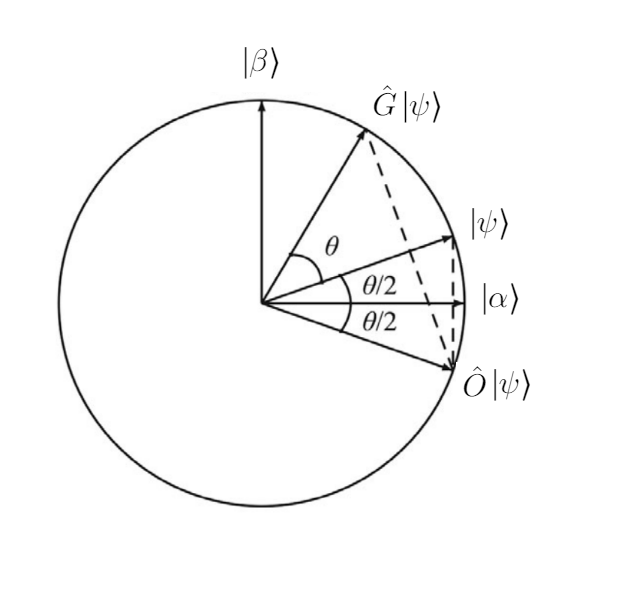
\includegraphics[width=0.6\textwidth]{Anexos/grover.png}
\caption{Grover}
\label{gr:Grover}
\end{figure}
donde $\text{CI}(x)$ es el entero completo de $x$, por ejemplo $\text{CI}(3,72)=3$. Tras aplicar $R$ veces el operador de Grover, el ángulo final sobre $\ket{\beta}$ es $<\pi/4$ y la probabilidad de medir un elemento marcado es significativa, $\pi^2/16>1/2$. El caso particular $M\ll N$ es notorio: $\theta/2\approx \sin(\theta/2)\approx \sqrt{M/N}$, con lo cual $R\approx N/M$, y el error después de la medición es $M/N$. \\
La complejidad del algoritmo es igual al número de rotaciones $R$, ya que cada aplicación tiene el costo de un solo llamado al oráculo. en (\ref{ec:RGrover}) $R$ tiene una cota superior $R=\lceil\pi/2\theta \rceil$, debido al máximo valor posible del numerador. Ahora, una cota inferior de $\theta$ impone otra cota superior sobre $R$.

\begin{equation}
    \frac{\theta}{2}>\sin\frac{\theta}{2}=\sqrt{\frac{M}{N}}
\end{equation}
Así que $R=\mathcal{O}(\frac{\pi}{4}\sqrt{\frac{N}{M}})$

Así que $R=\mathcal{O}(\sqrt{N/M})$ y en el caso de $M=1$, $R=\mathcal{O}(\sqrt{N})$.

\begin{center}
    \begin{tabular}{l}
    \hline \textbf{Algoritmo de Grover}\\\hline
    \textbf{entradas:} \\
    \textbf{salidas:}\\\hline
    \textbf{proceso}\\
    \textbf{1.} [Preparar:] Preparar el estado inicial $\ket{\psi}$ como en (\ref{ec:GroverInicial}).\\
\textbf{2.} Ejecutar lo siguiente $\mathcal{O}(\sqrt{N/M})$ número de veces:\\
(a) [Chequear:] Aplicar $\mathcal{O}$ (reflexión con respecto a $\ket{\alpha}$)\\
(b) [Actualizar:] Aplicar $2\ket{\psi}\bra{\psi}-I$ (reflexión con respecto a $\ket{\psi}$)\\
\textbf{3.} Medir el estado final\\\hline
    \end{tabular}{}
\end{center}{}
%Para el costo en la del algoritmo nos ocupamos del operador $(\ket{\psi}\bra{\psi}-I)$. En cuanto al oráculo sabemos que usarlo hace que el análisis de la eficiencia se base en el número de consultas, y que su implementación es particular al tipo de problema, así que aquí no nos ocupamos de él más allá de contar $R$.\\  Los pasos (1) y (3) tienen cada uno costo de $n$, por su parte, el paso (2) $N=\log n$.
Este algoritmo permite la solución a otros problemas además del de búsqueda exhaustiva de un elemento marcado en una base de datos, por ejemplo, encontrar posibles soluciones al problema del problema del viajante (traveling salesman problem)\footnote{"Dada una lista de ciudades y de distancias entre cada par de ellas, ¿cuál es la ruta más corta posible que visita cada ciudad y regresa a la ciudad de origen?"}, o el problema de distinción de los elementos resueltos por Ambainis.
%Este algoritmo fue probado como óptimo en la búsqueda de un elemento marcado.


\end{appendix}